\providecommand{\main}{../..}
\documentclass[\main/thesis.tex]{subfiles}

\begin{document}

\section{Cell Lineages}
In Figure \ref{fig:GeneralObservations_importantTimeStepsLineages} we show time-steps that are relevant to the major developmental stages of field cancerization, in particular we display the top twenty cell lineages at each of the time-steps.
\begin{figure}[H]
    \centering
    \begin{subfigure}[t]{.45\textwidth}
      \centering
      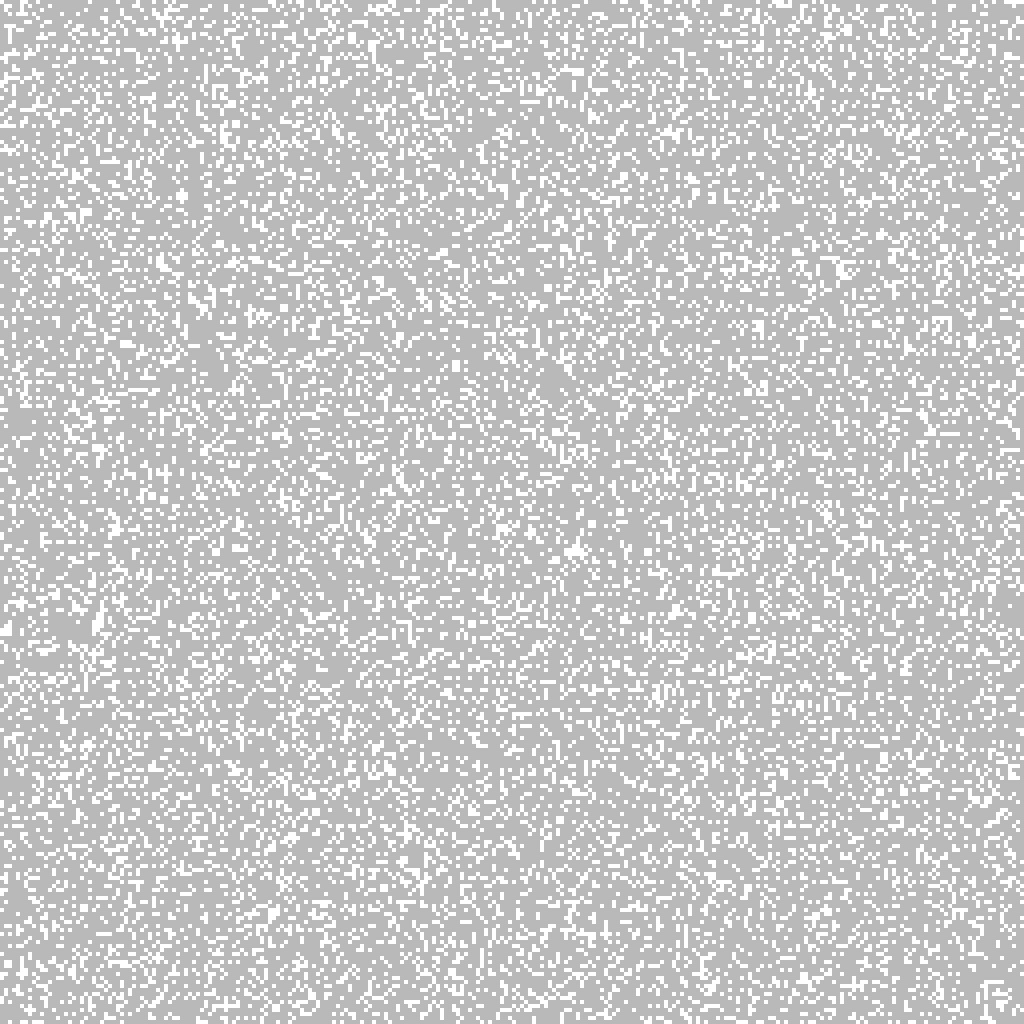
\includegraphics[width=\textwidth]{images/2_GeneralObservations/Fig6/1_init.jpeg}
      \caption{Initial seed}
      \label{fig:GeneralObservations_initSeedLineages}
    \end{subfigure}
    \begin{subfigure}[t]{.45\textwidth}
      \centering
      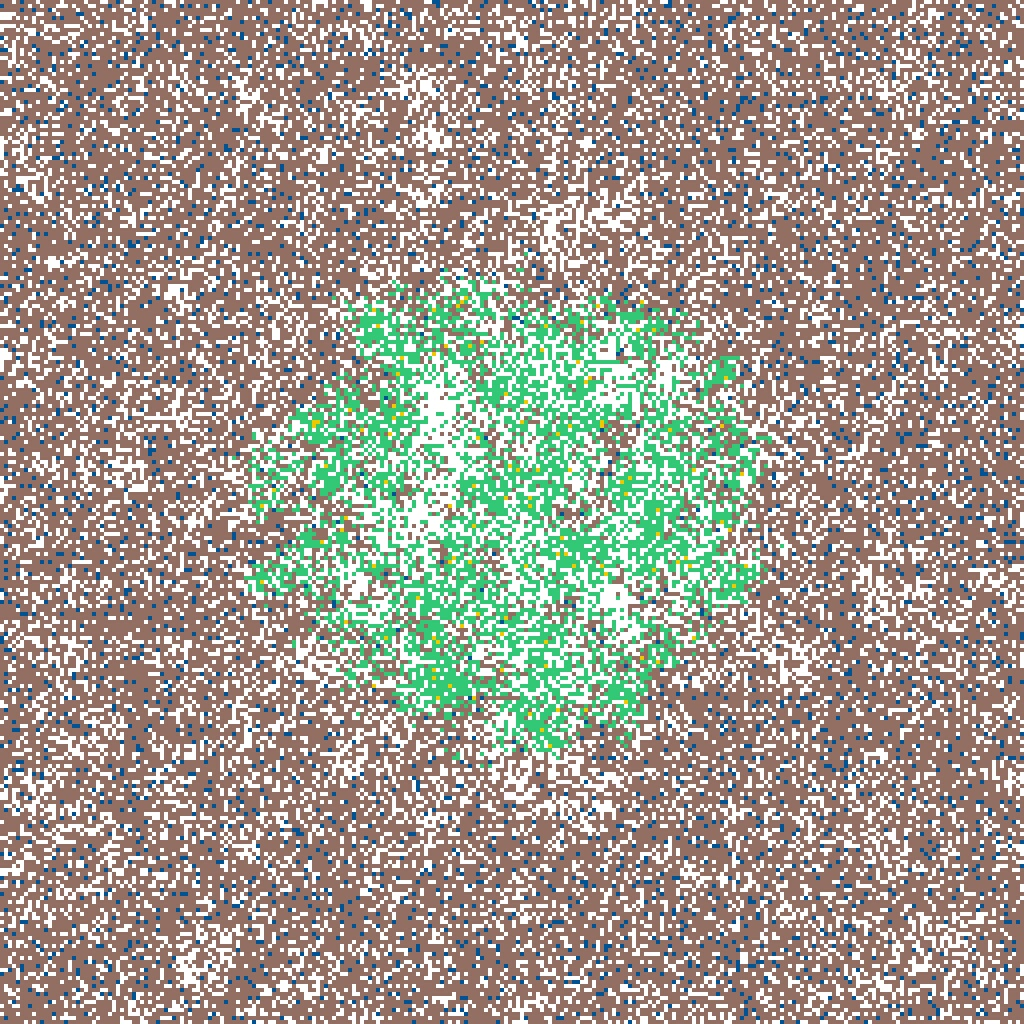
\includegraphics[width=\textwidth]{images/2_GeneralObservations/Fig6/2_early_field_1000.jpeg}
      \caption{Field early in its development}
      \label{fig:GeneralObservations_earlyFieldLineages}
    \end{subfigure}
    \begin{subfigure}[t]{.45\textwidth}
      \centering
      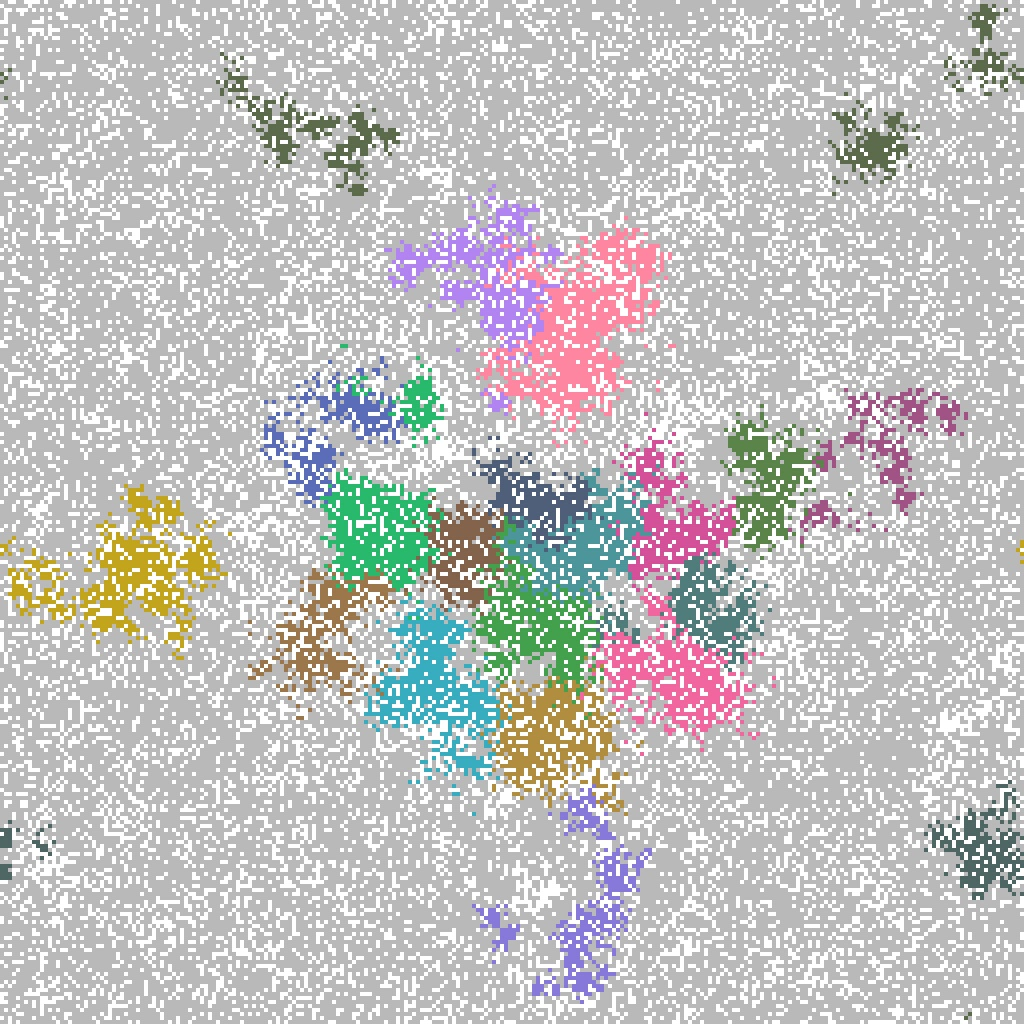
\includegraphics[width=\textwidth]{images/2_GeneralObservations/Fig6/3_late_field_1400.jpeg}
      \caption{Field later in its development prior to tumours}
      \label{fig:GeneralObservations_lateFieldLineages}
    \end{subfigure}
    \begin{subfigure}[t]{.45\textwidth}
      \centering
      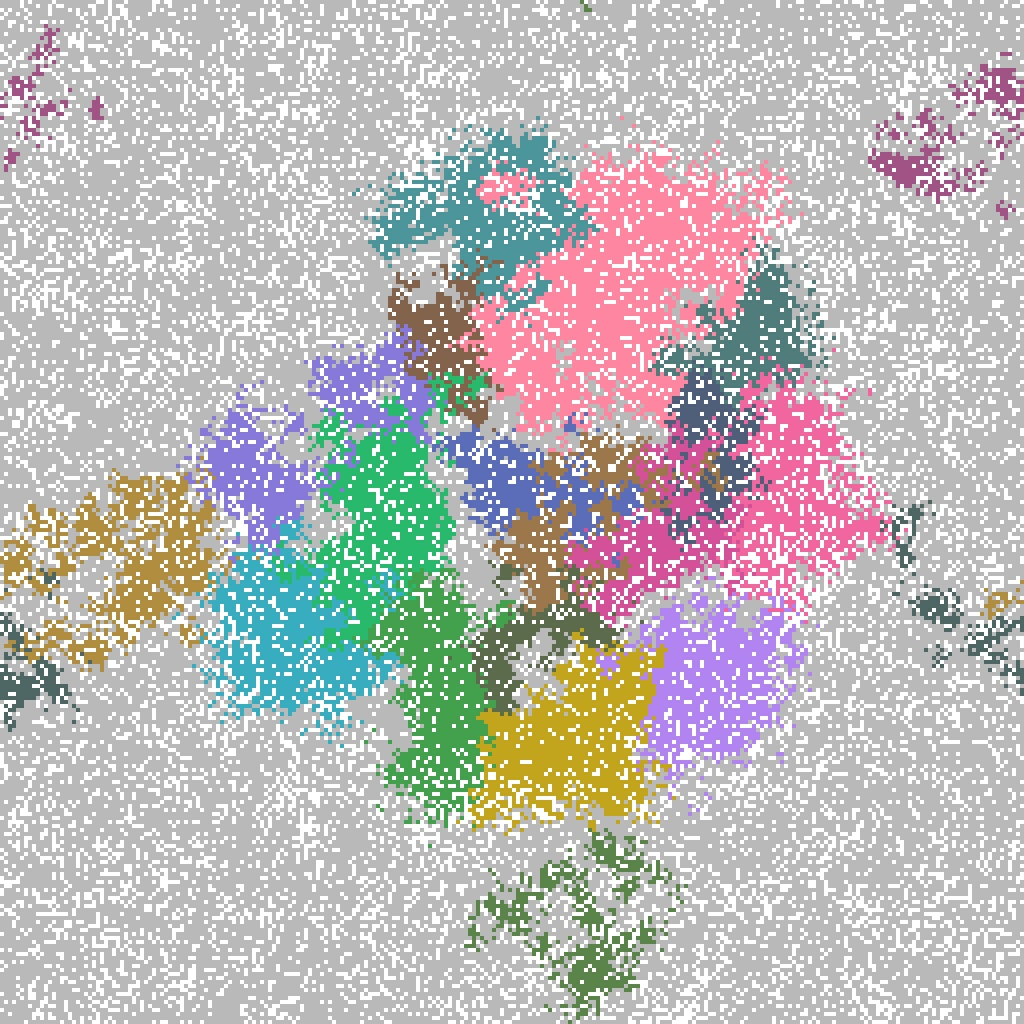
\includegraphics[width=\textwidth]{images/2_GeneralObservations/Fig6/4_early_tumour_1975.jpeg}
      \caption{Tumour masses early in their development}
      \label{fig:GeneralObservations_earlyTumourLineages}
    \end{subfigure}
    \begin{subfigure}[t]{.45\textwidth}
      \centering
      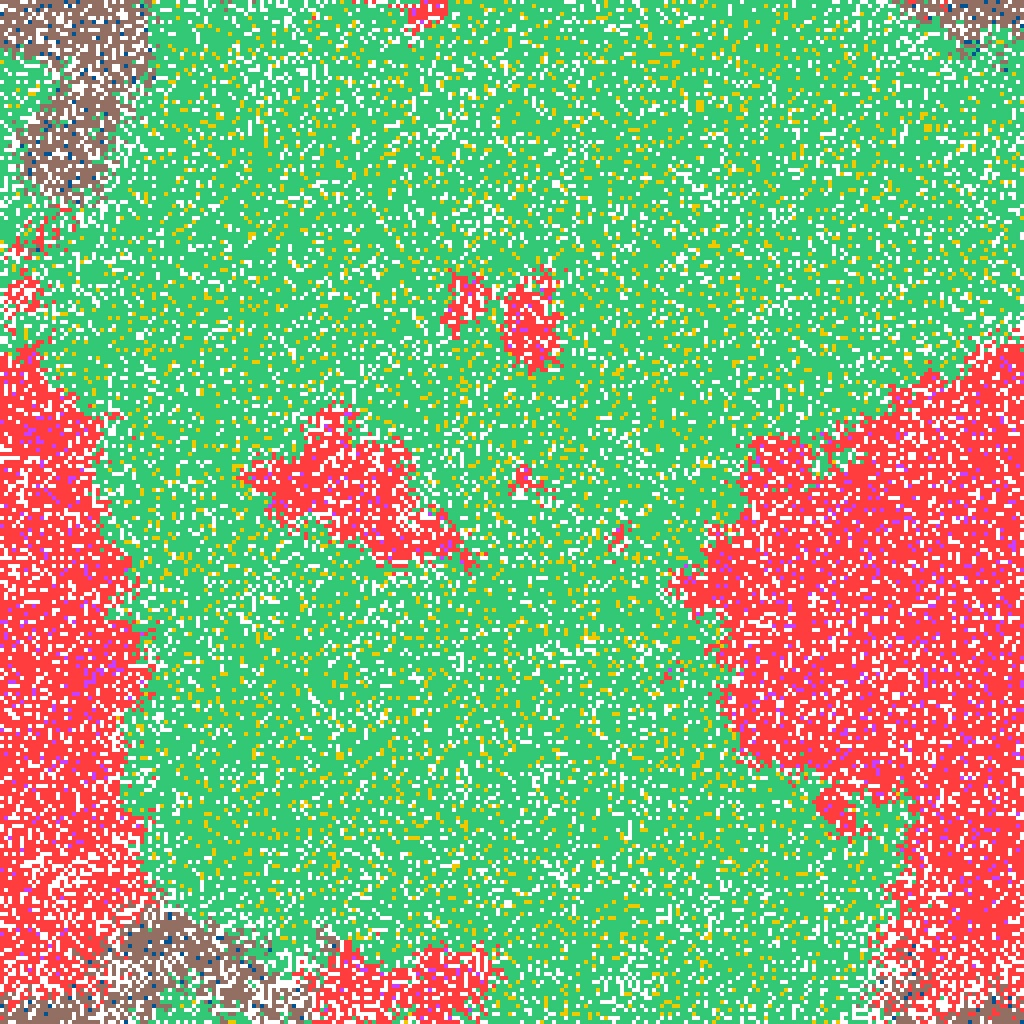
\includegraphics[width=\textwidth]{images/2_GeneralObservations/Fig6/5_late_tumour_3947.jpeg}
      \caption{Tumour masses later in their development}
      \label{fig:GeneralObservations_lateTumourLineages}
    \end{subfigure}
    \begin{subfigure}[t]{.45\textwidth}
      \centering
      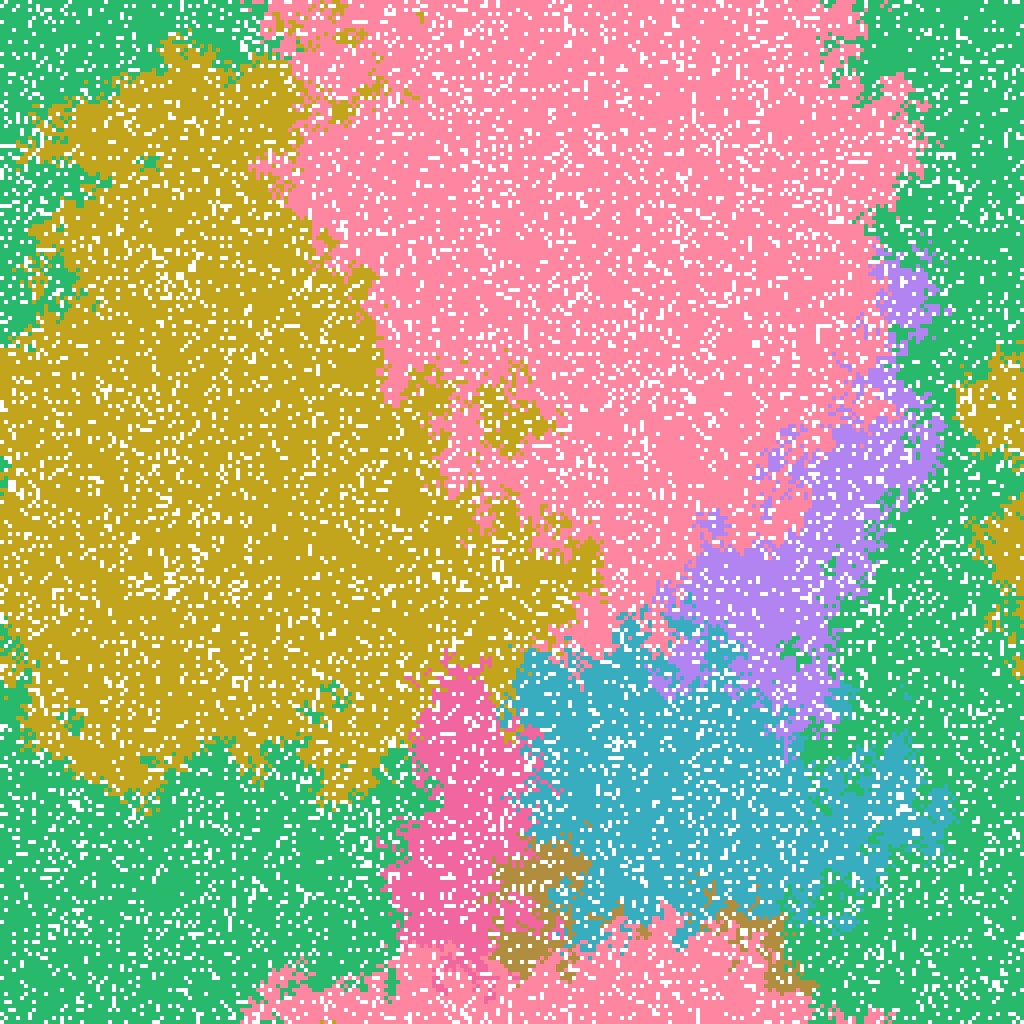
\includegraphics[width=\textwidth]{images/2_GeneralObservations/Fig6/6_final.jpeg}
      \caption{Final time-step}
      \label{fig:GeneralObservations_finalLineages}
    \end{subfigure}
    \caption{Important time-steps that show the top twenty lineages throughout the development stages of field cancerization. In the figures we show (a) the initial seed, (b) early cancer field formation, (c) later cancer field development, (d)-(f) cancer development. Note that light grey means the cell is not in any of the top twenty lineages and each colour represents a different cell lineage. 
    Parameters are as follows: grid size 256x256, carcinogen spatial distribution 2, both carcinogens activated.}
    \label{fig:GeneralObservations_importantTimeStepsLineages}
\end{figure}
In the figures we show (a) the initial seed, (b) early cancer field formation, (c) later cancer field development, in (d)-(f) cancer development. The initial seed does not have any lineages because we can not track lineages until after the first phenotypic actions occur. At the beginning of the field formation the largest cell lineages are scattered everywhere, but as the field develops and grows, the largest cell lineages are concentrated at the location of the field, as shown in Figure \ref{fig:GeneralObservations_earlyTumourLineages}. Note that the largest cell lineages increase in size as the field and tumour cells become more aggressive. Figure \ref{fig:GeneralObservations_importantTimeStepsLineages} shows that the cell lineages that are part of the field are the largest cell lineages in the domain, which goes to show that the field contains the most fit cells in the domain. By the final time-step the remaining lineages, less than ten, are all TC lineages. Initially, there are several cell lineages, but over time the number of cell lineages decreases as the higher fitness cell lineages overcome less fit lineages.

In Figure \ref{fig:MonoclonalvsPolyclonal_TumourLineages} we illustrate a time-step from a simulation that shows the largest tumour cell lineages, each represented by a different colour. We observe that most of the lineages are concentrated near the location of the carcinogen, with smaller lineages dispersed throughout the domain. Cell lineages are competitive as is demonstrated by tumour mass cell lines enveloping or infringing on other tumour mass cell lines, displayed in Figure \ref{fig:MonoclonalvsPolyclonal_TumourLineages}. Theoretically, given enough time the number of cell lineages would be reduced to one or very near to one, because certain cell lines become more and more competitive. Since we use periodic boundary conditions, we should be able to observe convergence to one lineage as time goes to infinity, this means our model will maintain multiple lineages only on sufficiently small space and time scales.
\begin{figure}[H]
    \centering
    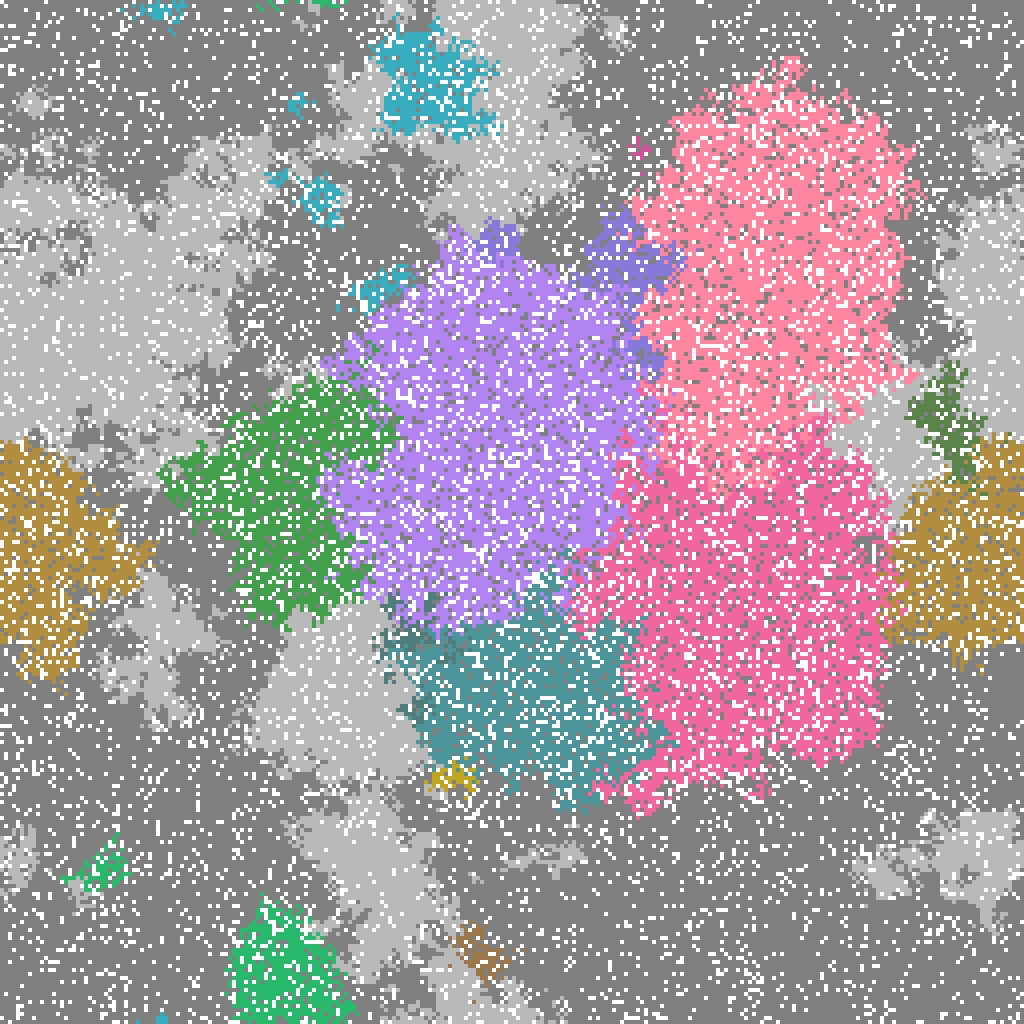
\includegraphics[width=\textwidth]{images/6_MonoclonalvsPolyclonal/Fig1/TumourLineages.jpeg}
    \caption{Each colour represents a different tumour cell lineage. Both the light green and light blue lineages have a main mass of tumour cells with other small masses disconnected from it, which implies they both have formed tumour masses by monoclonal origin. However, most of the tumour masses have been formed via polyclonal origin. Parameters are as follows: grid size 256x256, carcinogen spatial distribution 2, and both carcinogens activated.}
    \label{fig:MonoclonalvsPolyclonal_TumourLineages}
\end{figure}

\subsection{Monoclonal versus Polyclonal Origin}
We investigate whether a typical cancer field is formed via monoclonal or polyclonal origin. Our model demonstrated both, as evidenced by examining the tumour lineages over time in Figure \ref{fig:GeneralObservations_importantTimeStepsLineages}, where different cancer lineages are indicated in different colours. However, generally it seems that polyclonal origin is the more common origin of the tumour masses, as can be verified by Figure \ref{fig:MonoclonalvsPolyclonal_TumourLineages}.

The chance of monoclonal origin is associated with the amount of cell movement that occurs, since a cell has to move far away enough from its origin to form a new tumour mass. As a result, it is possible to increase the amount of monoclonal origin by increasing the chance of movement. Polyclonal origin has no relation to movement, thus it is much more likely to occur due to the vast amount of cells and competition between cell lineages. 

\end{document}